\documentclass{article}

% if you need to pass options to natbib, use, e.g.:
%     \PassOptionsToPackage{numbers, compress}{natbib}
% before loading neurips_2018

% ready for submission
% \usepackage{neurips_2018}

% to compile a preprint version, e.g., for submission to arXiv, add add the
% [preprint] option:
%     \usepackage[preprint]{neurips_2018}

% to compile a camera-ready version, add the [final] option, e.g.:
% \usepackage[final]{neurips_2018}

% to avoid loading the natbib package, add option nonatbib:
%     \usepackage[nonatbib]{neurips_2018}

\usepackage[utf8]{inputenc} % allow utf-8 input
\usepackage[T1]{fontenc}    % use 8-bit T1 fonts
\usepackage{hyperref}       % hyperlinks
\usepackage{url}            % simple URL typesetting
\usepackage{booktabs}       % professional-quality tables
\usepackage{amsfonts}       % blackboard math symbols
\usepackage{nicefrac}       % compact symbols for 1/2, etc.
\usepackage{microtype}      % microtypography
\usepackage{amsmath,amsfonts,amssymb}
\usepackage{graphicx}
\usepackage{enumerate}

\title{Report Assignment 1}

% The \author macro works with any number of authors. There are two commands
% used to separate the names and addresses of multiple authors: \And and \AND.
%
% Using \And between authors leaves it to LaTeX to determine where to break the
% lines. Using \AND forces a line break at that point. So, if LaTeX puts 3 of 4
% authors names on the first line, and the last on the second line, try using
% \AND instead of \And before the third author name.

\author{%
  Luc Weytingh
}

\begin{document}

\maketitle

\begin{abstract}
  insert abstracta
\end{abstract}

\section{Evaluating the gradients}

\subsection*{1.1a Linear Module}
\begin{align*}
  \frac{\partial L}{\partial W} \Rightarrow \left[\frac{\partial L}{\partial W}\right]_{ij} &= \frac{\partial L}{\partial W_{ij}}\\
                                                                                            &= \sum_{m,n}\frac{\partial L}{\partial Y_{mn}} \frac{\partial Y_{mn}}{\partial W_{ij}} \\
  &= \sum_{m,n}\frac{\partial L}{\partial Y_{mn}} \frac{\partial [XW^T + B]_{mn}}{\partial W_{ij}} \\
                                                                                            &= \sum_{m,n}\frac{\partial L}{\partial Y_{mn}} \frac{\partial}{\partial W_{ij}} \left(\sum_p X_{mp} (W^T)_{pn} + B_{mn}\right) \\
                                                                                            &= \sum_{m,n}\frac{\partial L}{\partial Y_{mn}} \frac{\partial}{\partial W_{ij}} \left(\sum_p X_{mp} W_{np} + B_{mn}\right) \\
                                                                                            &= \sum_{m,n}\frac{\partial L}{\partial Y_{mn}}  \sum_p X_{mp} \frac{\partial W_{np}}{\partial W_{ij}} \\
                                                                                            &= \sum_{m,n}\frac{\partial L}{\partial Y_{mn}}  \sum_p X_{mp} \delta_{ni}\delta_{pj} \\
                                                                                            &= \sum_{m,n}\frac{\partial L}{\partial Y_{mn}} X_{mj} \delta_{ni}
                                                                                              &= \sum_{m}\frac{\partial L}{\partial Y_{mi}} X_{mj}
\end{align*}

\begin{align*}
  \frac{\partial L}{\partial b} \Rightarrow \left[\frac{\partial L}{\partial b}\right]_i &= \frac{\partial L}{\partial b_i} \\
                                                                                         &= \sum_{m,n}\frac{\partial L}{\partial Y_{mn}} \frac{\partial Y_{mn}}{\partial b_i} \\
                                                                                         &= \sum_{m,n}\frac{\partial L}{\partial Y_{mn}} \frac{\partial [XW^T + B]_{mn}}{\partial b_i} \\
                                                                                         &= \sum_{m,n}\frac{\partial L}{\partial Y_{mn}} \frac{\partial}{\partial b_i}\left(\sum_p X_{mp}W_{np} + B_{mn}\right) \\
                                                                                         &= \sum_{m,n}\frac{\partial L}{\partial Y_{mn}} \frac{\partial B_{mn}}{\partial b_i} \\
                                                                                         &= \sum_{m,n}\frac{\partial L}{\partial Y_{mn}} \delta_{ni} \\
&= \sum_{m,n}\frac{\partial L}{\partial Y_{mi}}
\end{align*}


\begin{align*}
  \frac{\partial L}{\partial X} \Rightarrow \left[\frac{\partial L}{\partial X}\right]_{ij} &= \frac{\partial L}{\partial X_{ij}} \\
                                                                                         &= \sum_{m,n}\frac{\partial L}{\partial Y_{mn}} \frac{\partial Y_{mn}}{\partial X_{ij}} \\
                                                                                         &= \sum_{m,n}\frac{\partial L}{\partial Y_{mn}} \frac{\partial [XW^T + B]_{mn}}{\partial X_{ij}} \\
                                                                                            &= \sum_{m,n}\frac{\partial L}{\partial Y_{mn}} \frac{\partial}{\partial X_{ij}}\left(\sum_p X_{mp}W_{np} + B_{mn}\right) \\
                                                                                            &= \sum_{m,n}\frac{\partial L}{\partial Y_{mn}} \sum_p \frac{\partial X_{mp}}{\partial X_{ij}}W_{np} \\
                                                                                            &= \sum_{m,n}\frac{\partial L}{\partial Y_{mn}} \sum_p \delta_{mi}\delta_{pj}W_{np} \\
                                                                                            &= \sum_{m,n}\frac{\partial L}{\partial Y_{mn}} \delta_{mi}W_{nj} \\
  &= \sum_{n}\frac{\partial L}{\partial Y_{in}} W_{nj} \\
\end{align*}

\subsection*{1.1b Activation module}
\begin{align*}
  \frac{\partial L}{\partial X} \Rightarrow \left[\frac{\partial L}{\partial X}\right]_{ij} &= \frac{\partial L}{\partial X_{ij}} \\
                                                                                            &= \sum_{m,n}\frac{\partial L}{\partial Y_{mn}} \frac{\partial Y_{mn}}{\partial X_{ij}} \\
                                                                                            &= \sum_{m,n}\frac{\partial L}{\partial Y_{mn}} \frac{\partial h(X_{mn})}{\partial X_{ij}} \\
                                                                                            &= \sum_{m,n}\frac{\partial L}{\partial Y_{mn}} \frac{\partial [h(X)]_{mn}}{\partial X_{ij}} \\
                                                                                            &= \sum_{m,n}\frac{\partial L}{\partial Y_{mn}} \delta_{mi}\delta_{nj}\frac{\partial h(X_{mn})}{\partial X_{ij}} \\
                                                                                            &= \sum_{m}\frac{\partial L}{\partial Y_{mj}} \delta_{mi}\frac{\partial h(X_{mj})}{\partial X_{ij}} \\
  &= \frac{\partial L}{\partial Y_{ij}} \frac{\partial h(X_{ij})}{\partial X_{ij}} \\
\end{align*}

\subsection*{1.1c Softmax and Loss modules}
\begin{align*}
    \frac{\partial L}{\partial X} \Rightarrow \left[\frac{\partial L}{\partial X}\right]_{ij} &= \frac{\partial L}{\partial X_{ij}} \\
                                                                                            &= \sum_{m,n}\frac{\partial L}{\partial Y_{mn}} \frac{\partial Y_{mn}}{\partial X_{ij}} \\
                                                                                              &= \sum_{m,n}\frac{\partial L}{\partial Y_{mn}} \frac{\partial [Softmax(X)]_{mn}}{\partial X_{ij}} \\
                                                                                              &= \sum_{m,n}\frac{\partial L}{\partial Y_{mn}} \frac{\partial}{\partial X_{ij}} \left(\frac{e^{X_{mn}}}{\sum_ke^{X_{mk}}}\right)\\
                                                                                              &= \sum_{m,n}\frac{\partial L}{\partial Y_{mn}} \frac{\delta_{im}\delta_{jn}e^{X_{mn}}\sum_ke^{X_{mk}} - \delta_{im}e^{X_{ij}}e^{X_{mn}}}{\left(\sum_ke^{X_{mk}}\right)^2}\\
                                                                                              &= \sum_{m,n}\frac{\partial L}{\partial Y_{mn}} \frac{e^{X_{mn}}}{\sum_ke^{X_{mk}}} \left(\frac{\delta_{im}\delta_{jn}e^{X_{mn}}\sum_ke^{X_{mk}}}{\sum_ke^{X_{mk}}} - \frac{\delta_{im}e^{X_{ij}}e^{X_{mn}}}{\sum_ke^{X_{mk}}}\right)\\
                                                                                              &= \sum_{m,n}\frac{\partial L}{\partial Y_{mn}} \frac{e^{X_{mn}}}{\sum_ke^{X_{mk}}} \left(\delta_{im}\delta_{jn} - \frac{\delta_{im}e^{X_{ij}}e^{X_{mn}}}{\sum_ke^{X_{mk}}}\right)\\
  &= \sum_{n}\frac{\partial L}{\partial Y_{in}} Y_{in} \left(\delta_{jn} - Y_{ij}\right)\\
\end{align*}


\section{2 PyTorch MLP}
\subsection{2.1}
The training en testing procedures yield a 0.48 accuracy with the default parameters. The loss and accuracy curves for this model can be found in Figure \ref{fig:loss_accuracy}.

\begin{figure}[h!]
    \centering
    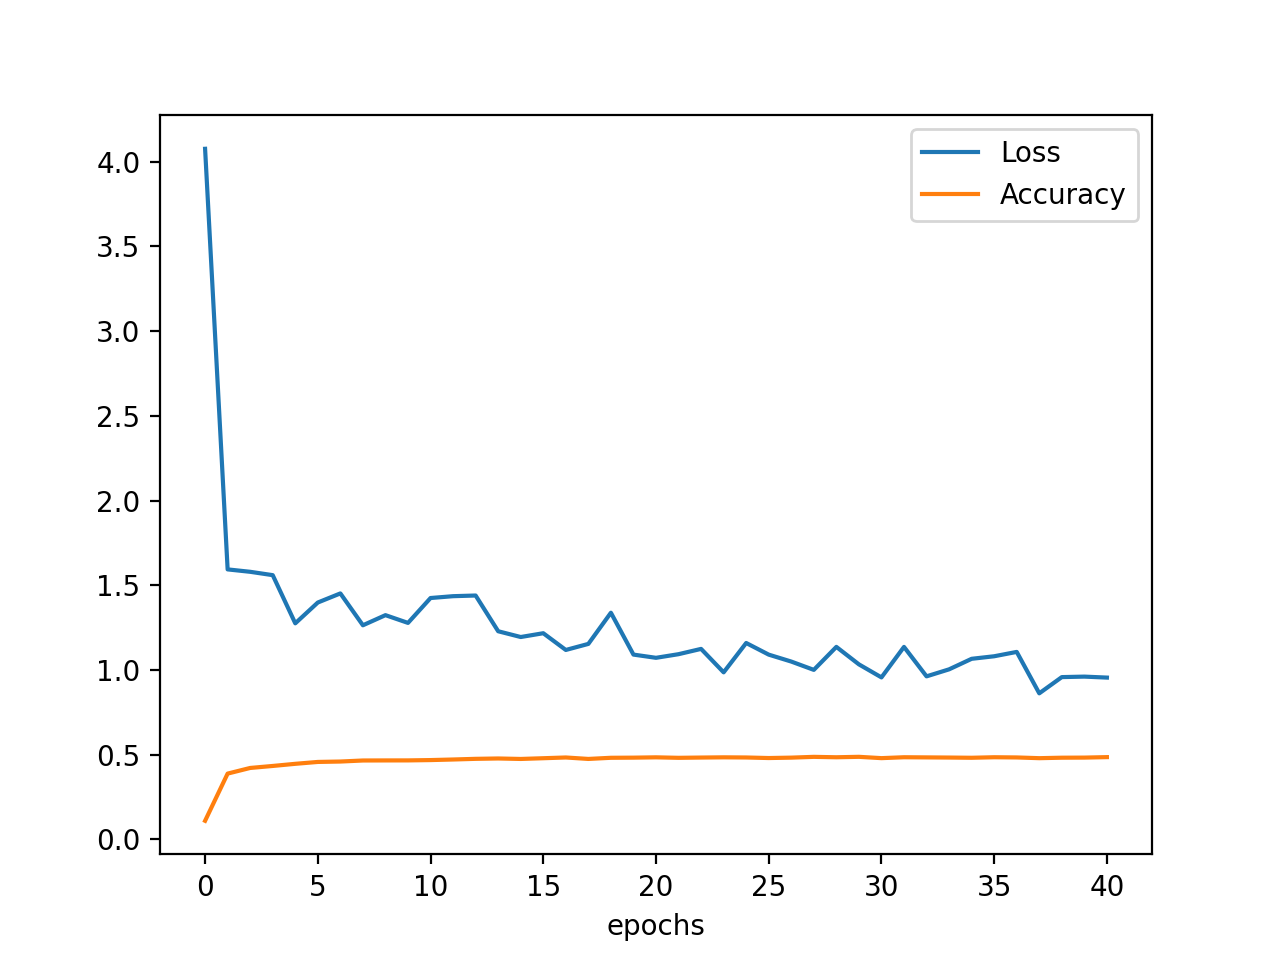
\includegraphics[width=1.0\textwidth]{loss_accuracy.png}
    \caption{The loss and accuracy for a MLP with default parameters and 3 hidden layers of size 40, 50, and 40.}
    \label{fig:loss_accuracy}
\end{figure}

\end{document}